% LaTeX file for resume
% This file uses the resume document class (res.cls)

\documentclass{res}
\usepackage{fullpage}
\usepackage{hyperref}
\usepackage{graphicx}

\hypersetup{
  colorlinks = true,
  linkcolor=blue,   % color of internal links
  citecolor=blue,   % color of links to bibliography
  urlcolor=blue,    % color of external links
  pagebackref=true,
  implicit=false,
  bookmarks=true,
  bookmarksopen=true,
  pdfdisplaydoctitle=true
}

% the margin option causes section titles to appear to the left of body text
\textwidth=5.75in % increase textwidth to get smaller right margin
%\usepackage{helvetica} % uses helvetica postscript font (download helvetica.sty)
%\usepackage{newcent}   % uses new century schoolbook postscript font

\begin{document}

\name{Matthew R. Goodman } % the \\[12pt] adds a blank line after name

\address{{\bf Home} \\ Mission District \\ San Francisco, CA 94110 \\ 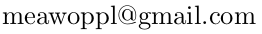
\includegraphics[scale=1.5]{email-address.png} \\ \href{https://meawoppl.github.io}{meawoppl.github.io}}

\address{{\bf Work} \\ 2051 Harrison St. \\ San Francisco, CA 94110 \\ (415) 234-3549 }

\begin{resume}

\section{Objective}
Be a force for world betterment via incremental measured change.

\section{Work Experience and Leadership}

{\bf CEO \& Co--Founder,} \href{http://www.exclosure.io}{Exclosure} \hfill
Nov 2021 -- Present
\begin{itemize}  \itemsep -2pt
  \item Founded company, raised capital, recruited early team.
  \item Created worldwide space monitoring network based on small optical telescopes.
  \item Bid and won FFP contracts with NOAA/DOC for commercial space tracking pilot.
  \item Accepted into TAP Lab and Catalyst accelerator programs funded by US SpaceForce.
  \item Proposed, won, and executed AFWERX STTR project.
\end{itemize}

{\bf Technical Mercenary,} Various \hfill
2019 -- 2021
\begin{itemize}  \itemsep -2pt
  \item {\bf Starfish Neuroscience} -- Aided in the design, build, and prototype of a transcranial
        focused ultrasound stimulation device. Roles ranged from simulation \& modeling to
        mechanical, electrical, acoustic, integration and testing. Lead significant investigation
        of human skull geometry variation investigation across a large population.
  \item {\bf Endiatx} -- Implemented, in Verilog, complete image acquisition, compression, and radio
        transmission for ingestible pill robot. Advised electrical design for extremely power limited application.
        Integration testing and EE flex design bring-up and testing.
  \item {\bf Arizona Optical Metrology} -- Build high performance computational optics design software
        for the translation of designs to reified VLSI mask artwork.
        Replaced existing tool with complete back-compatibility, 10,000x speed increase and enhanced accuracy.
        Built OSS GDSII tooling optimized for the JVM ecosystem.
\end{itemize}

{\bf CTO \& Co--Founder,} \href{http://www.3scan.com}{3Scan} \hfill
May 2011 -- May 2019
\begin{itemize}  \itemsep -2pt
  \item Lead data intensive biotech startup from foundation to merger with Strateos
  \item Grew the organization through four doublings of staff, from 4 to 80+
  \item Hired, managed, and developed ICs and leads, totaling $> 60$ engineers.
  \item Worked with cofounders, board, VCs, leads, and pharma partners to provide strategic vision,
    technical roadmap, and product delivery
  \item Managed creation of high performance $(\approx 50 \mathrm{Gb/s})$, big-data $(> 10\mathrm{PB})$ tooling for
    storage, analysis, and visualization of 3d histological data
\end{itemize}

{\bf President,}  \href{http://coupdefoud.re}{Coup De Foudre} \hfill   Fall 2015 -- Present
\begin{itemize} \itemsep -2pt
  \item Created and lead a high-voltage technical arts troupe
  \item Delivered Burning Man 2019 Honorarium art project ``Theophany''
  \item Incorporated and maintained a 501c3 charity structure
  \item Curate relationships with donors, museums, and grantees
  \item Portfolio: \href{https://meawoppl.github.io/portfolio.html}{https://meawoppl.github.io/portfolio.html}
\end{itemize}

{\bf Scientific Data Analyst,} \href{https://www.atimetals.com/}{ATI Allvac} \hfill
Summer 2007 -- Summer 2008
\begin{itemize} \itemsep -2pt
  \item Unified huge body of process data from several databases for purposes of ML application
  \item Developed tools for engineers and analysts to model casting/forging processes
  \item Automated process simulation of solidification for process control and improvement
  \item Datamining and scientific data analysis for plant process improvement 
      resulted in large cost savings by predictive/preventive maintenance
\end{itemize}

{\bf Consultant,} PACE Metallography, ATI Allvac, Phoenix Heat Treating \hfill Various

{\bf Graduate Researcher,} \href{https://www.utexas.edu/}{University of Texas at Austin} \hfill
Fall 2010 -- Fall 2012
\begin{itemize} \itemsep -2pt
  \item Computational modeling and imaging analysis of the primary visual cortex of primates
  \item Development of machine learning techniques for medical recommendation systems
  \item Literal monkey wrangling
\end{itemize}

{\bf Graduate Research Assistant,} \href{https://www.arizona.edu/}{University of Arizona} \hfill
Fall 2008 -- Spring 2010
\begin{itemize} \itemsep -2pt
  \item Modeled heat and mass transfer for NASA/ESA space solidification experiments on ISS
  \item Developed HPC CFD solver for solidification, microfluidics, and biological systems
  \item Worked with ISS payload operations on-site in Huntsville Alabama 
\end{itemize}

{\bf Project Leader,}  \href{https://seds.arizona.edu/}{SEDS} ``Rockoon''  project \hfill   Fall 2008 -- Spring 2010
\begin{itemize} \itemsep -2pt
  \item Led team of two--dozen undergraduates in interdisciplinary design project
  \item Responsible for FAA Clearances and safety of high-altitude high-power rocketry
\end{itemize}

{\bf President,} \href{https://ceramics.org/members/member-communities/classes/keramos}{Keramos} \& {\bf Vice--President,} Material Advantage \hfill Fall 2007 -- Spring 2008
\begin{itemize} \itemsep -2pt
  \item Provided tutoring, and social organization
  \item Lead $\approx10$ students in outreach, teaching, and grant-writing.
  \item Keramos Awarded ``Most Improved Chapter'' in 2008
\end{itemize}

{\bf Treasurer -- President,} h+ Tucson \hfill Fall 2007 -- Spring 2008
\begin{itemize} \itemsep -2pt
  \item Organized a technoprogressive journal club
  \item This group became \href{http://hplusmagazine.com/}{\textit{h+ magazine}}
\end{itemize}

{\bf MSE Laboratory TA/Preceptor,} University of Arizona \hfill Fall 2007 -- Spring 2008
\begin{itemize} \itemsep -2pt
  \item MSE 414 -- Solidification of Castings -- Ran aluminum casting laboratory
  \item MSE 223 -- Materials Processing -- Taught three groups of 5--7 about materials processing
  \item MSE 110 -- Solid State Chemistry -- Oversaw MSE related lab activities
\end{itemize}

{\bf Barista,} Starbucks \hfill Fall 2005 -- Fall 2008

\section{Patents \& Publications}

  F\,Aeffner, M\,Zarella, N\,Buchbinder, M\,Bui, \textbf{M\,Goodman}, 
  D\,Hartman, G\,Lujan, M\,Molani, A\,Parwani, K\,Lillard, O\,Turner,
  V\,Vemuri, A\,Yuil-Valdes, and D\,Bowman
  ``Introduction to Digital Image Analysis in Whole-slide Imaging''
  \href{http://www.jpathinformatics.org/temp/JPatholInform1019-318182_000518.pdf}{Digital Pathology Association, 2019.}

  \textbf{M\,Goodman}, T\,Huffman, C\,Daniel
  ``Spatial multiplexing of histological stains''
  \href{https://patents.google.com/patent/US20170011511A1/en}{US Patent App.\,15/205,288}

  C\,Daniel, \textbf{M\,Goodman}, K\,Sean, T\,Huffman
  ``Methods and apparatuses for sectioning and imaging samples''
  \href{https://patents.google.com/patent/US20160290895A1/en}{US Patent App.\,15/084,186}

  S\,Raghavan, \textbf{M\,Goodman}, T\,Huffman, C\,Daniel, C\,Monteith, J\,Kwon
  ``Internet-connected high-throughput and high-resolution three-dimensional tissue scanner to
  enable large-scale automated histology''
  \href{https://doi.org/10.1109/IST.2016.7738254}{Imaging Systems and Techniques (IST), 2016.}

  \textbf{M\,Goodman}, C\,Daniel
  ``Motion strategies for scanning microscope imaging''
  \href{https://patents.google.com/patent/US20150138532A1/en}{US Patent App.\,14/529,503}

  C\,Sung, Y\,Choe, \textbf{M\,Goodman}, T\,Huffman,
  ``Scalable, Incremental Learning for Cell Detection in High-Throughput 3D Microscopy Data''
  \href{https://doi.org/10.1109/IJCNN.2013.6706769}{International Joint Conference on Neural Networks 2013.}

  AG\,Hendrick, RG\,Erdmann, \textbf{MR\,Goodman},
  ``Practical Considerations for Selection of Representative
  Elementary Volumes for Fluid Permeability in Fibrous Porous Media,''
  \href{http://dx.doi.org/10.1007/s11242-012-0051-8}{Transport in Porous Media.\,Volume 94.\,2012.}

  \textbf{MR\,Goodman}
  ``Brain--Machine Interfaces'' -- Chapter 26 of \textit{New Materials and Technologies For Healthcare.}
  \href{http://amzn.com/1848165587}{ISBN: 978-1848165588.} 2012.

  RG\,Erdmann, AG\,Hendrick, and \textbf{MR\,Goodman}
  ``Properties of Stochastic Permeability,''
  \href{http://dx.doi.org/10.1007/s12666-009-0038-5}{Transactions of the Indian Institute of Metals. 2011.}

\section{News \& Publications}
  ``An operating system for the biology lab'' \\
  \href{https://www.nature.com/articles/d41586-019-02875-z}{\textbf{Nature Outlook}} \hfill Sept.\,2019

  ``Three-dimensional Imaging and Scanning: Current and Future Applications for Pathology'' \\
  \href{https://www.ncbi.nlm.nih.gov/pmc/articles/PMC5609355/}{\textbf{Journal of Pathology Informatics}} \hfill Sept.\,2017
  
  ``3Scan raises \$14 million for a robotic microscope that could accelerate drug discovery'' \\
  \href{https://techcrunch.com/2016/07/11/3scan-raises-14-million-for-a-robotic-microscope-that-could-accelerate-drug-discovery/
  }{\textbf{TechCrunch}} \hfill July 2016
  
  ``Digital Imaging On The Cutting Edge Of Tissue Analysis'' \\
  \href{https://www.forbes.com/sites/joshwolfe/2015/01/28/digital-imaging-on-the-cutting-edge-of-tissue-analysis/}{\textbf{Forbes}} \hfill Jan.\,2015
  
  ``Mapping brain circuitry with a light microscope'' \\
  \href{https://www.ncbi.nlm.nih.gov/pmc/articles/PMC3982327/}{\textbf{Nature Methods}} \hfill June\,2013
  
\section{Presentations}
  ``Cloud Pathology''
  [re:Invent] Cloud Computing for Biotech R\&D \hfill Oct.\,2018

  ``New Approaches for Volumetric Pathology.''
  MICCAI COMPAY \href{https://sites.google.com/site/compaysymposium2018/speakers}{2018 Workshop} \hfill Sept.\,2018

  ``Digital Pathology Challenges''
  Vision Industry and Technology Forum \hfill Dec.\,2017

  ``Make Dangerous Art''
  Ignite Talks \hfill Sept.\,2017

  ``The Physics of Tesla Coils and Swing-Sets''
  Ignite Talks \hfill Sept.\,2016

  ``10 Tools for Everything''
  Lightning talk at SciPy \hfill June\,2012

\section{Education}
  PhD.\,Biomedical Engineering (Incomplete) \\
  \href{https://www.bme.utexas.edu/}{University of Texas at Austin}
  
  M.S.\,Materials Science and Engineering,
  (GPA 3.83/4.0) \\
  Thesis: \href{http://hdl.handle.net/10150/193422}{``Properties of Stochastic Flow and Permeability of Random Porous Media''} \\
  \href{https://mse.engineering.arizona.edu/}{University of Arizona}, Tucson, AZ
  
  B.S.\,Materials Science and Engineering (In major GPA 3.55/4.0) \\
  \href{https://mse.engineering.arizona.edu/}{University of Arizona}, Tucson, AZ

% I don't think anyone cares about this any more...
\section{Academic Honors}
UT -- NIH NRSA Fellowship for Imaging Science and Informatics \hfill 2010--2011 \\
UA -- Dean’s List \hfill 2007--2008 \\
UA -- ASM International -- Darko Babic Scholarship \hfill 2007--2008 \\
UA -- College of Engineering -- Award for Academic Distinction \hfill 2005--2008 \\
UA -- College of Engineering -- Departmental Honors for Outstanding Achievement \hfill 2005--2006

\section{Languages and Tools}
 \begin{tabular}{l p{5.5in}}
   \underline{Fluent in:}    & English, Python, Java, c, Verilog, AWS/GCP, \LaTeX \\
   \underline{Useful with:}  & Typescript/Javascript, Rust, Docker, c++, LLVM-IR, CUDA, Scala \\
   \underline{Under duress:} & Japanese, FORTRAN, qBasic, php, sql, RoR, bash, Meteor, MATLAB \\
   \underline{Novice at:}    & Golang, Kotlin, Electron, React Native, Unity
 \end{tabular}

\section{Miscellaneous}
  \begin{tabular}{l p{5.5in}}
    \underline{OSS Contributions:} & cPython, numba, scipy, pandas, OpenCV, libcamera, esp-idf, \\
                                   & pycuda, datadog, emscripten, progressbar, mingds  \\
    \underline{Interests:}         & Brain-Machine Interfaces, Plasma Physics, Rock Climbing, woodworking,\\
                                   & Blacksmithing and Casting, High Power Electronics, EDA Software, \\
                                   & Abstract Algebra, Group-Theory, Quasicrystals, Satellites, Astronomy, \\
                                   & SciFi, Writing, Bicycles, Computational Geometry, Timelapse Photography
 \end{tabular}

\end{resume}
\end{document}
